\documentclass[aspectratio=141,10pt]{beamer}

% Look of the lecture slides: white, dark red titles, grey text
\usepackage[T1]{fontenc}
\usepackage[scaled=0.92]{helvet}
\renewcommand{\familydefault}{\sfdefault}
\usepackage{amsmath,amssymb}
\usepackage{booktabs,colortbl,array}
\usepackage{graphicx}
\usepackage{tikz}

\definecolor{aimsred}{HTML}{990000}
\definecolor{rowpink}{HTML}{F7E9E9}
\definecolor{textgrey}{HTML}{404040}
\definecolor{s1col}{HTML}{C0442A}
\definecolor{s2col}{HTML}{3A6FBF}

\usetheme{default}
\setbeamertemplate{navigation symbols}{}
\setbeamercolor{normal text}{fg=textgrey,bg=white}
\setbeamercolor{structure}{fg=aimsred}
\setbeamerfont{frametitle}{series=\bfseries,size=\Large}
\setbeamertemplate{frametitle}{\vskip0.8em\centering\usebeamerfont{frametitle}\color{aimsred}\insertframetitle\par\vskip0.2em}
\setbeamertemplate{itemize item}{\color{aimsred}$\bullet$}
\setbeamertemplate{footline}{\hfill\color{textgrey}\footnotesize\insertframenumber\hspace{1em}\vspace{0.6em}}

\newcommand{\callout}[2]{%
  \begin{center}\fcolorbox{aimsred}{rowpink!60}{\begin{minipage}{#1}\centering #2\end{minipage}}\end{center}}
\newcommand{\hl}[1]{{\bfseries\color{aimsred}#1}}
\newcommand{\R}{\mathcal R_0}

% Image with a coordinate system on top: (0,0) bottom left, (1,1) top right
\newenvironment{annotimg}[2]{%
  \begin{tikzpicture}%
  \node[anchor=south west,inner sep=0] (img) at (0,0) {\includegraphics[width=#1]{#2}};%
  \begin{scope}[x={(img.south east)},y={(img.north west)}]\ignorespaces}
  {\end{scope}\end{tikzpicture}\ignorespacesafterend}
\tikzset{note/.style={overlay,font=\scriptsize\bfseries,text=aimsred,fill=white,fill opacity=0.85,text opacity=1,inner sep=1.5pt,align=center},
         arr/.style={overlay,->,>=stealth,thick,aimsred}}

\begin{document}

% =====================================================================
% 1. Title and objective
% =====================================================================
\begin{frame}[plain]
\centering
\vspace{0.2em}

\includegraphics[height=2.1cm]{img/logo1.png}\\[1.3em]
{\Large\bfseries\color{aimsred} Project 3: Stochastic versus deterministic models of\\[0.2em]
endemic and multi-strain infections}\\[1.4em]
\fcolorbox{aimsred}{rowpink!60}{\begin{minipage}{0.92\textwidth}\sloppy\hyphenpenalty=10000\exhyphenpenalty=10000
\textbf{\color{aimsred}Objective.} Use Python simulations to illustrate the type of behaviour that results from compartmental deterministic ODE models and from SSA (Stochastic Simulation Algorithm).\\[0.6em]
Then compare the two approaches and explain how they help us understand disease processes.
\end{minipage}}\\[1.6em]

\includegraphics[height=1.1cm]{img/logo2.png}\hspace{1.5cm}

\includegraphics[height=0.85cm]{img/logo3.png}\hspace{1.5cm}

\includegraphics[height=0.75cm]{img/logo0.png}
\end{frame}

% =====================================================================
% 2. SIRS compartment model
% =====================================================================
\begin{frame}{Compartment model: cartoon diagram}
\begin{columns}[c]
\column{0.38\textwidth}
\textbf{\color{aimsred}Dynamical system (SIRS)}
\[
\begin{aligned}
\frac{dS}{dt}&=-\beta SI+\omega R\\[0.3em]
\frac{dI}{dt}&=\beta SI-\gamma I\\[0.3em]
\frac{dR}{dt}&=\gamma I-\omega R
\end{aligned}
\]
\small
\begin{itemize}\setlength\itemsep{0.3em}
  \item State $\mathbf x=[S,I,R]$, \ $N=S+I+R$ fixed.
  \item The three equations add up to zero.
  \item New arrow $R\to S$: loss of immunity.
\end{itemize}
\column{0.60\textwidth}
\centering
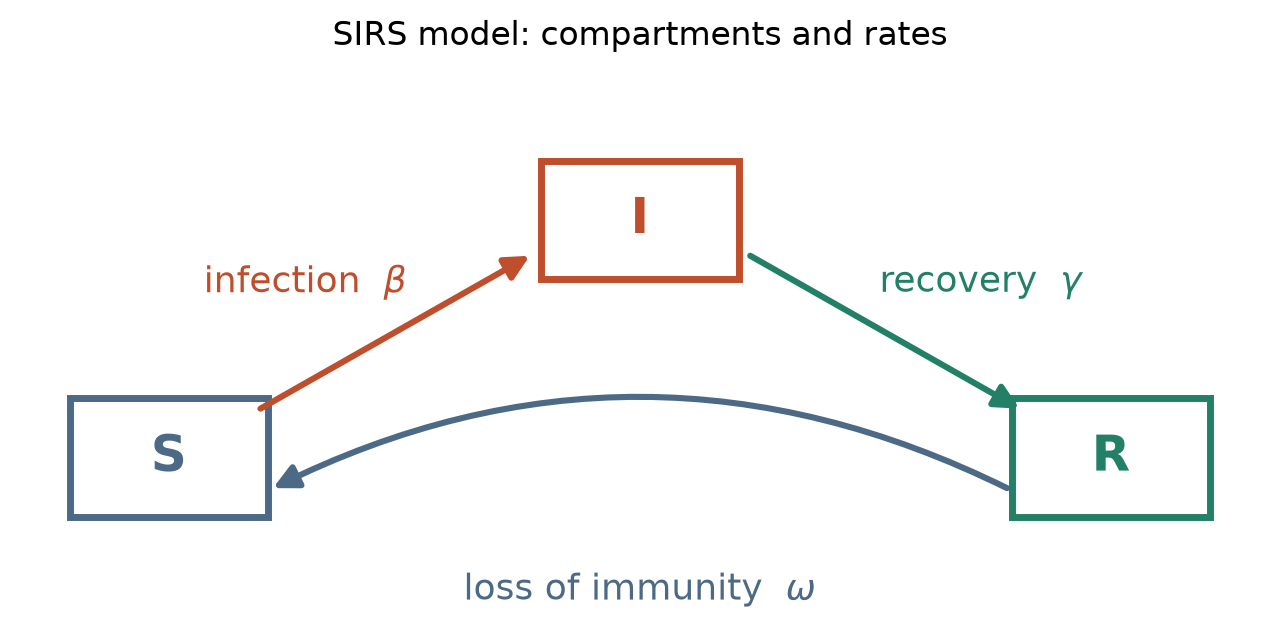
\includegraphics[width=\textwidth]{img/s2_cartoon_rates.png}
\end{columns}
\end{frame}

% =====================================================================
% 3. Events and propensities
% =====================================================================
\begin{frame}{Events, state change vectors, propensities}
\centering
\renewcommand{\arraystretch}{1.6}
\begin{tabular}{l c c c}
\rowcolor{aimsred}\color{white}\bfseries Event & \color{white}\bfseries Reaction & \color{white}\bfseries Vector $[\Delta S,\Delta I,\Delta R]$ & \color{white}\bfseries Propensity $a_j(\mathbf x)$\\
Infection & $S+I\to 2I$ & $[-1,+1,\;0]$ & $\beta\,S\,I$\\
\rowcolor{rowpink} Recovery & $I\to R$ & $[\;0,-1,+1]$ & $\gamma\,I$\\
Loss of immunity & $R\to S$ & $[+1,\;0,-1]$ & $\omega\,R$\\
\end{tabular}
\\[1.4em]
\raggedright
\begin{itemize}\setlength\itemsep{0.9em}
  \item Loss of immunity is a first order event, like cell death on the propensity slide of the CME lecture ($X_i\to$ products, $a=k\,x_i$).
  \item Each of the $R$ people loses immunity at rate $\omega$, so $a_3=\omega R$. The mean immune time is $1/\omega$.
  \item Infection uses the mass action form $k\,x_ix_j$ from the same slide, so no division by $N$.
\end{itemize}
\end{frame}

% =====================================================================
% 4. Equilibria
% =====================================================================
\begin{frame}{Two equilibria and a critical population size}
\begin{columns}[T]
\column{0.44\textwidth}
\textbf{\color{aimsred}Disease free}\\[0.4em]
$I^*=0,\ R^*=0,\ S^*=N$\\[0.3em]
It always exists.\\[1.4em]
\textbf{\color{aimsred}Endemic}\\[0.4em]
$S^*=\dfrac{\gamma}{\beta}$, and from $N=S^*+I^*+R^*$:
\[ N=\frac{\gamma}{\beta}+I^*\Big(1+\frac{\gamma}{\omega}\Big) \]
\column{0.52\textwidth}
\centering
\fcolorbox{aimsred}{rowpink!60}{\begin{minipage}{0.95\columnwidth}\centering
$\displaystyle I^*=\frac{\omega}{\omega+\gamma}\Big(N-\frac{\gamma}{\beta}\Big)$\\[1.0em]
$\displaystyle R^*=\frac{\gamma}{\omega+\gamma}\Big(N-\frac{\gamma}{\beta}\Big)$\end{minipage}}\\[1.0em]
\raggedright
$I^*>0$ exactly when
\[ N>N_c=\frac{\gamma}{\beta}\qquad\Big(\R=\frac{\beta N}{\gamma}>1\Big) \]
\end{columns}
\vspace{0.8em}
\callout{0.75\textwidth}{\large\bfseries\color{aimsred}With the project values, $N_c=0.15/0.01=15$.}
\end{frame}

% =====================================================================
% 4. Numerical ODE solutions
% =====================================================================
\begin{frame}{Numerical ODE solutions}
\vspace{-0.6em}
\centering
% Row 1: below the threshold, plus the table and the comments
\begin{minipage}[c]{0.50\textwidth}
\centering
{\footnotesize\bfseries\color{aimsred} $N\le 15$ (below $N_c$): the infection dies out}\\[0.15em]
\begin{annotimg}{0.49\textwidth}{img/s4_ode_N10.png}
  \node[note] (t) at (0.45,0.50) {dies out};
  \draw[arr] (t.south) -- (0.42,0.21);
\end{annotimg}\hfill
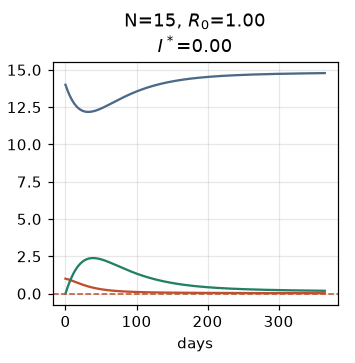
\includegraphics[width=0.49\textwidth]{img/s4_ode_N15.png}
\end{minipage}\hfill
\begin{minipage}[c]{0.47\textwidth}
\scriptsize
\renewcommand{\arraystretch}{1.25}\setlength{\tabcolsep}{3.5pt}
\centering
\begin{tabular}{l r r r r r}
\rowcolor{aimsred}\color{white}$N$ & \color{white}10 & \color{white}20 & \color{white}30 & \color{white}50 & \color{white}100\\
$I^*$ theory & 0 & 0.71 & 2.14 & 5.00 & 12.14\\
\rowcolor{rowpink} $I$ from ODE (long run) & 0 & 0.71 & 2.14 & 5.00 & 12.14\\
\end{tabular}\\[0.6em]
\raggedright\footnotesize
\begin{itemize}\setlength\itemsep{0.3em}
  \item \hl{$N=10$:} the infection dies out.
  \item \hl{$N>15$:} an epidemic peak, then damped oscillations toward $I^*$ (dashed line).
  \item The numerics match the analysis. Close to $N_c$ the approach is slow.
\end{itemize}
\end{minipage}\\[0.3em]
% Row 2: above the threshold
{\footnotesize\bfseries\color{aimsred} $N>15$: an epidemic peak, then damped oscillations toward $I^*$}\\[0.15em]
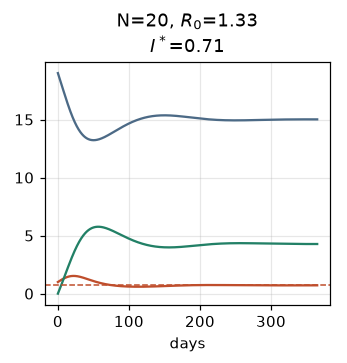
\includegraphics[width=0.315\textwidth]{img/s4_ode_N20.png}\hfill
\begin{annotimg}{0.315\textwidth}{img/s4_ode_N50.png}
  \node[note] (p) at (0.62,0.79) {epidemic peak};
  \draw[arr] (p.west) -- (0.23,0.45);
  \node[note] (d) at (0.60,0.67) {damped oscillations $\to I^*$};
  \draw[arr] (d.south) -- (0.36,0.28);
\end{annotimg}\hfill
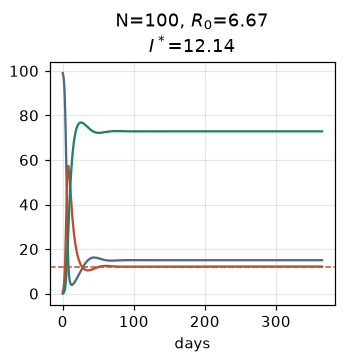
\includegraphics[width=0.315\textwidth]{img/s4_ode_N100.png}
\end{frame}

% =====================================================================
% 5. SSA runs against the ODE
% =====================================================================
\begin{frame}{SSA runs against the ODE}
\vspace{-0.7em}
\begin{columns}[c,totalwidth=1.06\textwidth]
\column{0.74\textwidth}
\centering
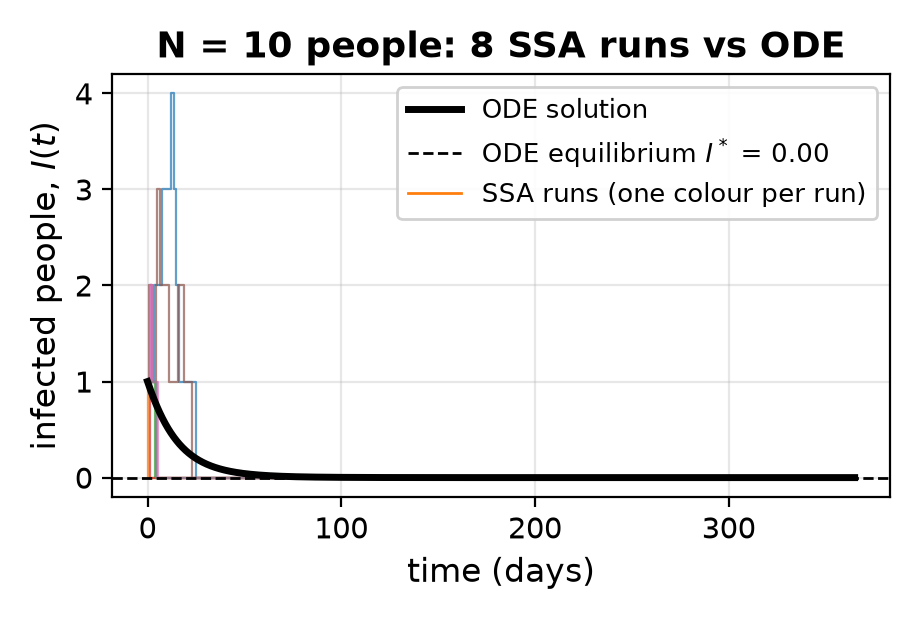
\includegraphics[width=0.495\linewidth]{img/s5_ssa_labelled_N10.png}\hfill
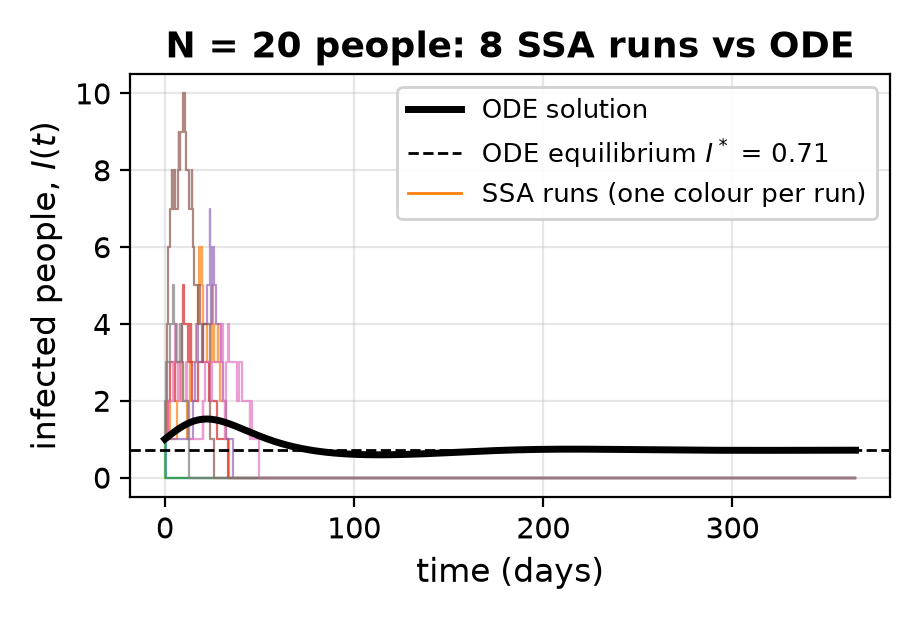
\includegraphics[width=0.495\linewidth]{img/s5_ssa_labelled_N20.png}\\[0.3em]
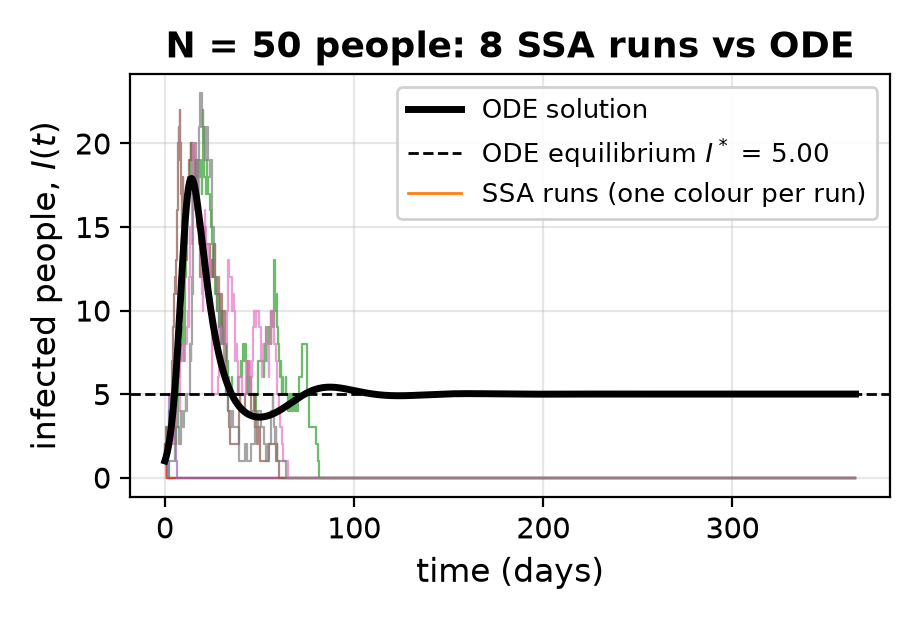
\includegraphics[width=0.495\linewidth]{img/s5_ssa_labelled_N50.png}\hfill
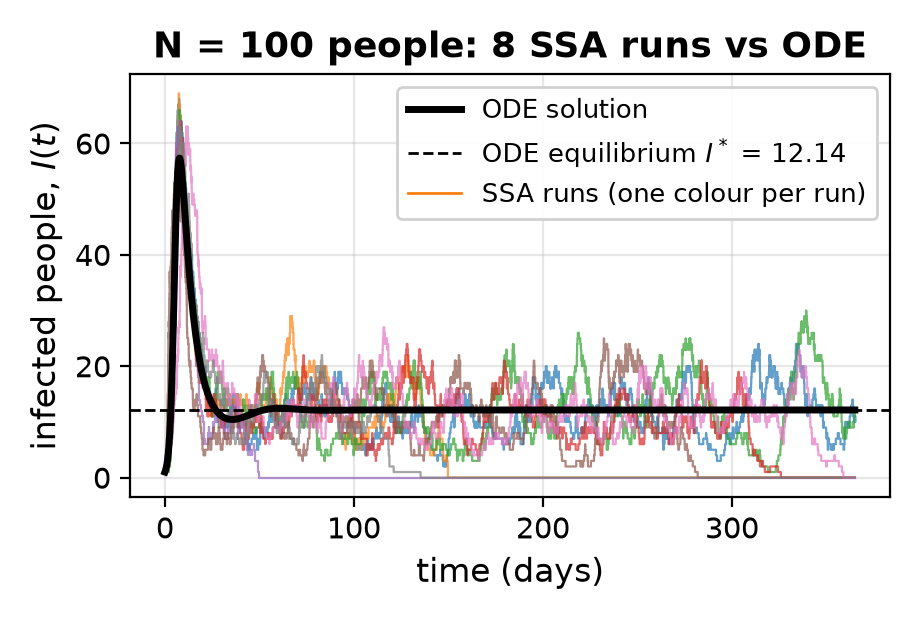
\includegraphics[width=0.495\linewidth]{img/s5_ssa_labelled_N100.png}
\column{0.30\textwidth}
\footnotesize
\begin{itemize}\setlength\itemsep{0.8em}
  \item \hl{Black:} ODE and its equilibrium $I^*$. \hl{Colours:} eight stochastic runs.
  \item \hl{$N=10<N_c$:} both models agree, the infection dies out within a month.
  \item \hl{$N=20$ and $N=50$:} all eight runs end at $I=0$, while the ODE stays endemic.
  \item \hl{$N=100$:} some runs keep fluctuating around the ODE level.
\end{itemize}
\end{columns}
\end{frame}

% =====================================================================
% 6. Two strain model
% =====================================================================
\begin{frame}{Two-strain model with waning immunity}
\vspace{-0.5em}
\begin{columns}[c]
\column{0.33\textwidth}
\textbf{\color{aimsred}\small Dynamical system}\\[-0.4em]
{\scriptsize
\[
\begin{aligned}
\dot S&=\mu(1-S)-\beta_1SI_1-\beta_2SI_2\\&\quad+\omega_1R_1+\omega_2R_2\\
\dot I_1&=\beta_1(S+R_2)I_1-(\gamma_1+\mu)I_1\\
\dot I_2&=\beta_2(S+R_1)I_2-(\gamma_2+\mu)I_2\\
\dot R_1&=\gamma_1I_1-\beta_2R_1I_2-(\omega_1+\mu)R_1\\
\dot R_2&=\gamma_2I_2-\beta_1R_2I_1-(\omega_2+\mu)R_2
\end{aligned}
\]}
{\scriptsize Proportions: $S+I_1+I_2+R_1+R_2=1$.}
\column{0.65\textwidth}
\centering
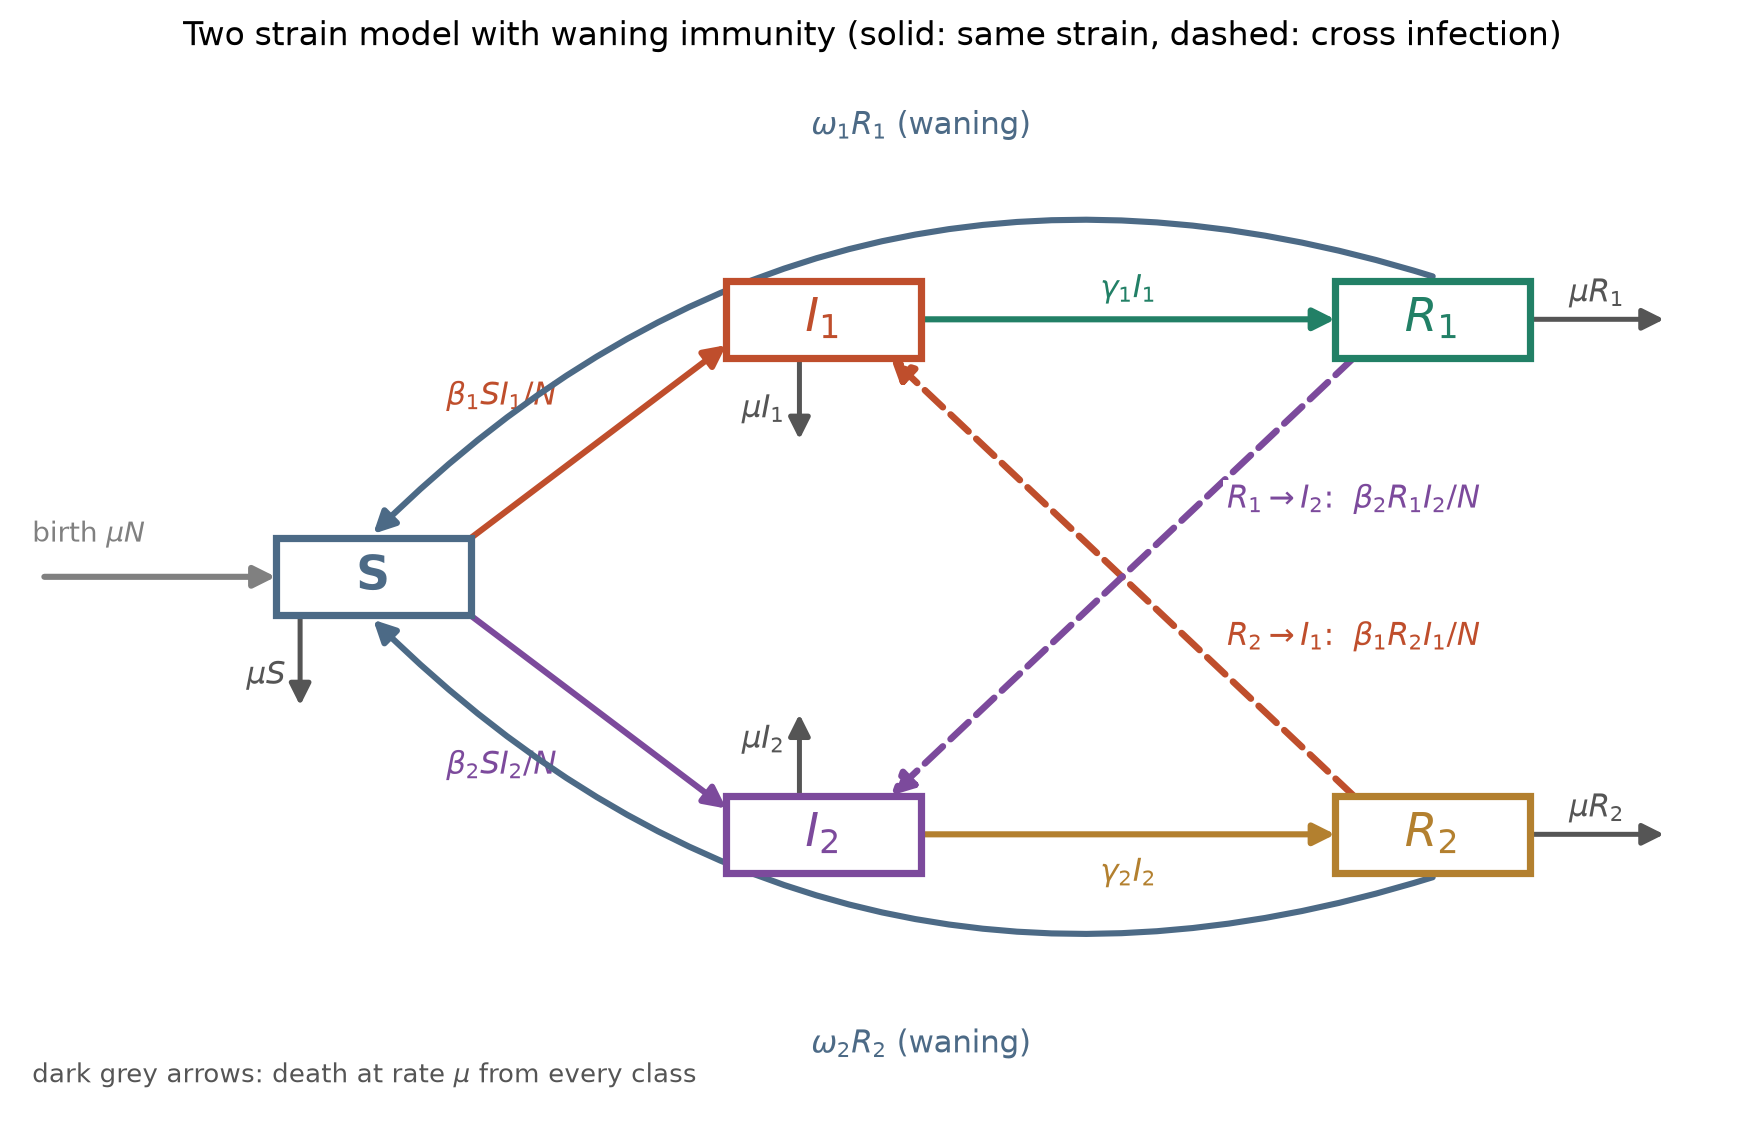
\includegraphics[width=\textwidth]{img/p2fig1.png}
\end{columns}
\vspace{0.1em}
\fcolorbox{aimsred}{rowpink!60}{\begin{minipage}{0.95\textwidth}\centering
\textbf{\color{aimsred}Reduced system} \ (eliminate $S=1-I_1-I_2-R_1-R_2$)\\[-0.3em]
\[
\begin{aligned}
\dot I_1&=\beta_1(1-I_1-I_2-R_1)I_1-(\gamma_1+\mu)I_1, &\qquad \dot R_1&=\gamma_1I_1-\beta_2R_1I_2-(\omega_1+\mu)R_1\\
\dot I_2&=\beta_2(1-I_1-I_2-R_2)I_2-(\gamma_2+\mu)I_2, &\qquad \dot R_2&=\gamma_2I_2-\beta_1R_2I_1-(\omega_2+\mu)R_2
\end{aligned}
\]
\end{minipage}}
\end{frame}

% =====================================================================
% 7. ODE vs. SSA
% =====================================================================
\begin{frame}{ODE vs.\ SSA}
\vspace{-0.6em}
\centering
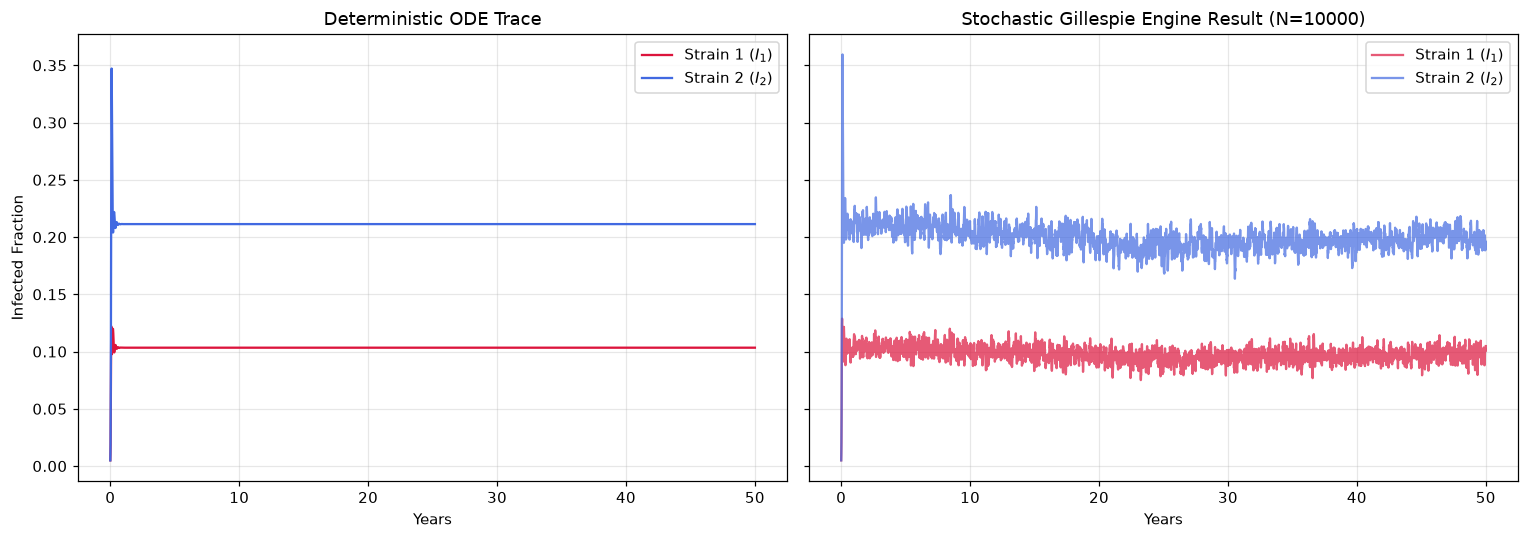
\includegraphics[width=0.93\textwidth]{img/p2fig2.png}\\[0.1em]
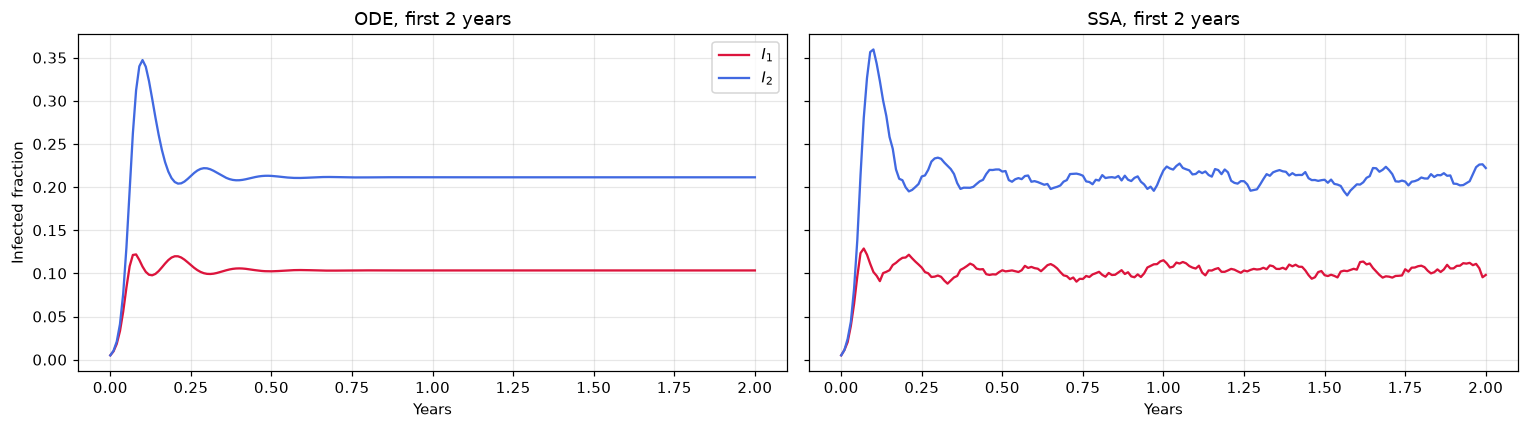
\includegraphics[width=0.93\textwidth]{img/p2fig3.png}\\[-0.1em]
{\footnotesize $N=10{,}000$, 50 years. Bottom row: zoom on the first 2 years.}
\end{frame}

% =====================================================================
% 8. Graphical outcomes
% =====================================================================
{\setbeamerfont{frametitle}{series=\bfseries,size=\large}
\begin{frame}{Graphical outcomes of the ODE and the Gillespie simulations}
\vspace{-0.4em}
\begin{columns}[c,totalwidth=1.06\textwidth]
\column{0.23\textwidth}
\centering
\fcolorbox{s1col}{white}{\begin{minipage}{0.92\columnwidth}\centering
{\bfseries\color{s1col}Strain 1}\\[0.2em]
$\displaystyle \R^{1}=\frac{\beta_1}{\gamma_1+\mu}$\\[0.4em]
$=\dfrac{120}{52.02}=\mathbf{2.31}$
\end{minipage}}\\[1.0em]
\fcolorbox{s2col}{white}{\begin{minipage}{0.92\columnwidth}\centering
{\bfseries\color{s2col}Strain 2}\\[0.2em]
$\displaystyle \R^{2}=\frac{\beta_2}{\gamma_2+\mu}$\\[0.4em]
$=\dfrac{100}{26.02}=\mathbf{3.84}$
\end{minipage}}\\[1.0em]
{\scriptsize Both $\R>1$. One run with $N=300$ people.}
\column{0.81\textwidth}
\centering
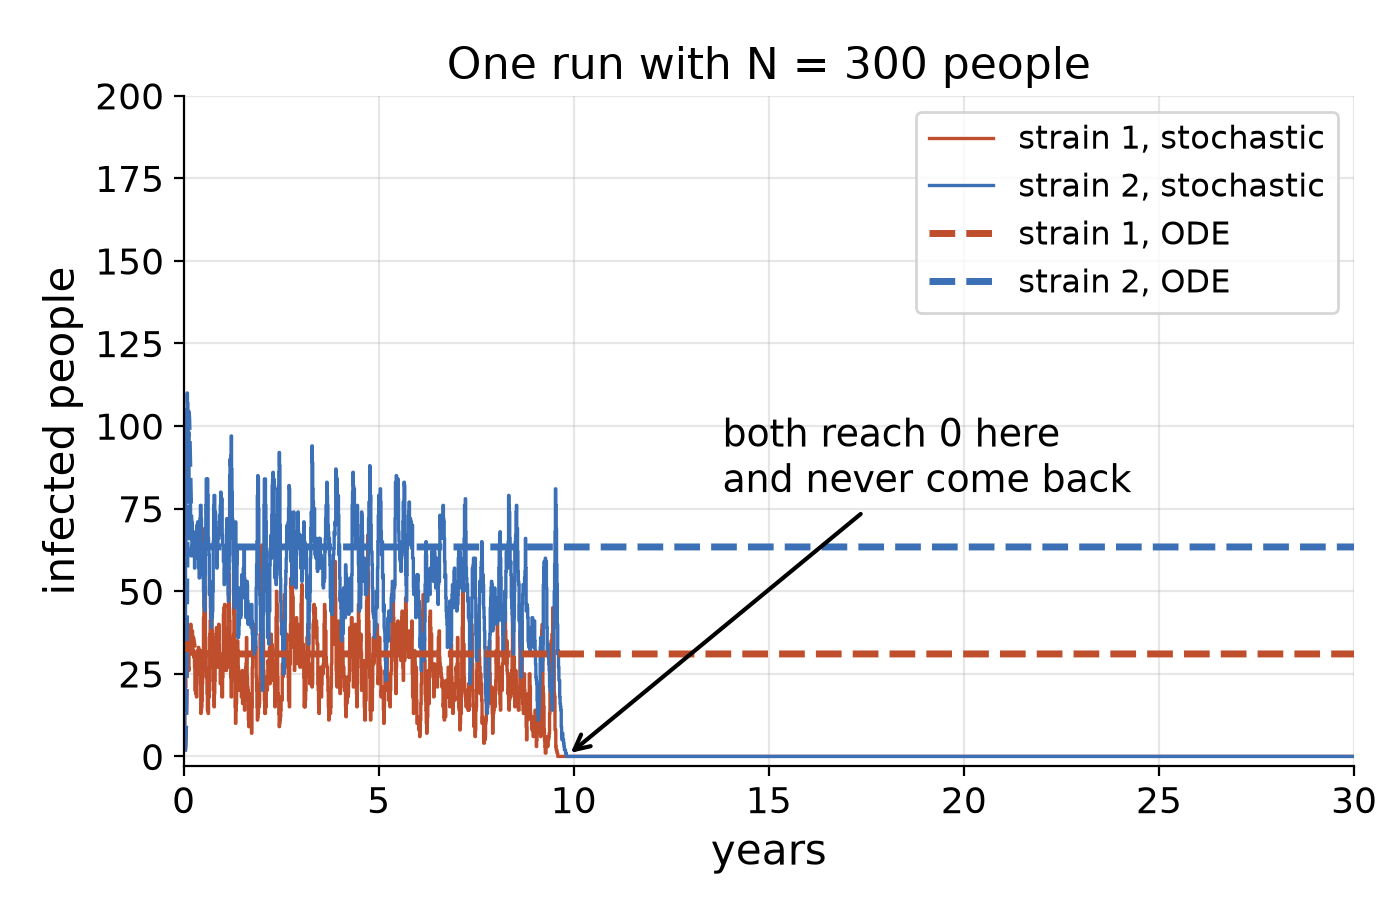
\includegraphics[width=\columnwidth]{img/s8_N300.png}
\end{columns}
\vspace{-0.2em}
\callout{0.95\textwidth}{\textbf{Conclusion:} the ODE settles at a non-zero level for both strains, but in the stochastic run the strains do not coexist: both reach 0 near year 10 and never come back.}
\end{frame}
}

% =====================================================================
% 10. Conclusion
% =====================================================================
\begin{frame}{Remarks}
\large
\begin{itemize}\setlength\itemsep{1.4em}
  \item ODE: for $N\le15$ the model enters the disease free state. For $N>15$ it enters the endemic state.
  \item ODE: both strains coexist at a stable endemic level ($\R^1=2.31$, $\R^2=3.84$).
  \item $\R>1$ is necessary for the disease to persist.
\end{itemize}
\vspace{1.2em}
\callout{0.9\textwidth}{Deterministic models tell us the level at which a disease settles. Stochastic models tell us whether it actually survives.}
\end{frame}

% =====================================================================
% 11. Thank you
% =====================================================================
\begin{frame}[plain]
\centering
\vspace{0.4em}

\includegraphics[height=2.1cm]{img/logo1.png}\\[1.4em]
{\fontsize{40}{44}\selectfont\bfseries\color{aimsred} Thank you!}\\[1.4em]
\callout{0.8\textwidth}{\large We sincerely thank \textbf{\color{aimsred}Prof.\ Nick} for the guidance\\[0.2em] and support throughout this project.}
\vspace{0.6em}
{\small\bfseries\color{aimsred}Group members}\\[0.3em]
{\small OGOUNCHI Géraud \quad$\cdot$\quad Fombo-Nfoba Mary \quad$\cdot$\quad Emmanuel Donkor\\[0.2em]
Ramsford Ganyo \quad$\cdot$\quad Raphael AMOH}\\[1.2em]

\includegraphics[height=1.1cm]{img/logo2.png}\hspace{1.5cm}

\includegraphics[height=0.85cm]{img/logo3.png}\hspace{1.5cm}

\includegraphics[height=0.75cm]{img/logo0.png}
\end{frame}

\end{document}
